%!!! cambiar esto por el diagrama de visio cuando este :)
\pagebreak
\section{Cursograma de Compras}
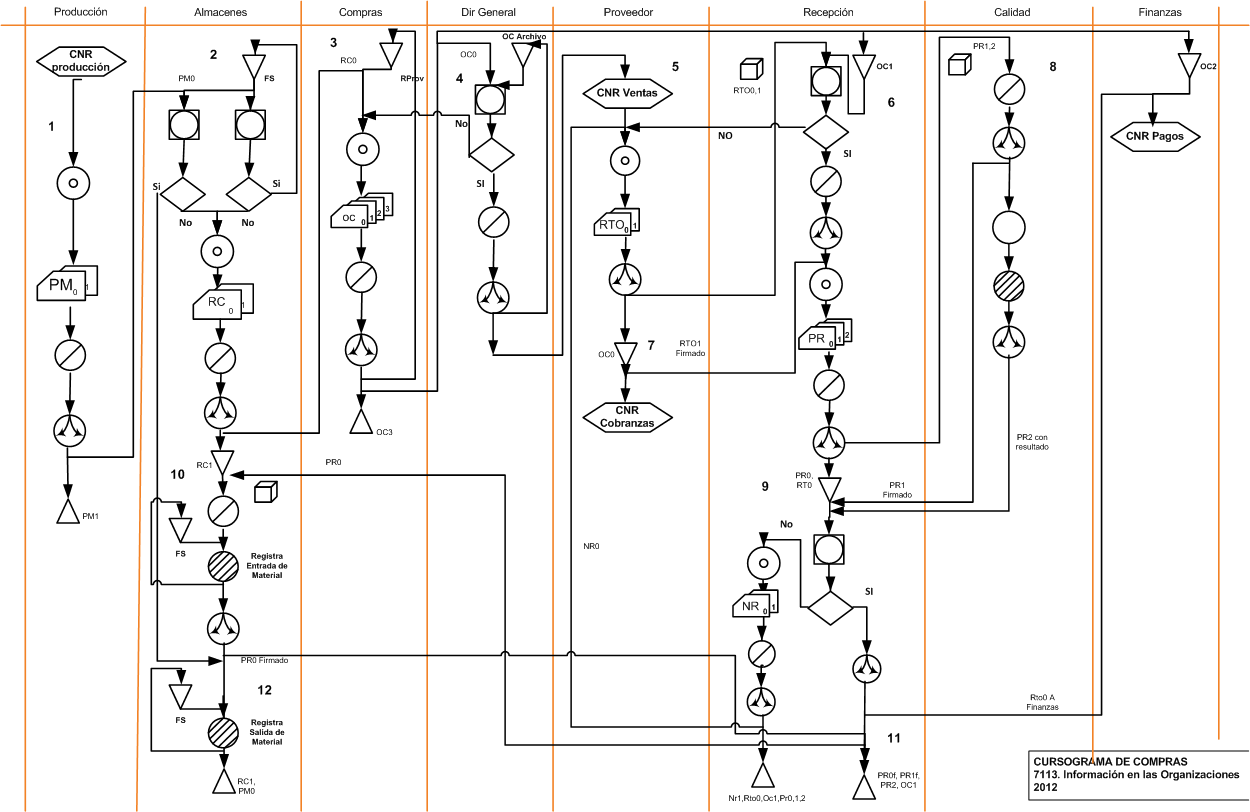
\includegraphics [scale=0.5 ,angle=90]{Empresa/Circuitos/Compras/Compras-Procedimiento.png}

\pagebreak
\section{Procedimiento de Compras}
\begin{description}
\item[1 - Producción] Tras detectar necesidad de materiales el sector de Producción emite un Pedido de Materiales (PM) en original y copia, el nivel autorizante firma el original y lo envía al sector de Almacenes, archiva la copia.
\item[2 - Almacenes] Tras recibir Pedido de Materiales del sector de Producción, Almacenes chequea las existencias y si tiene materiales suficientes los despacha; si no tiene los materiales necesarios, o se alcanza el punto de pedido, Almacenes emite un Requerimiento de Compra (RC) en original y copia, lo firma y envía al sector de Compras el original archivando la copia.
\item[3 - Compras] Recibido el Requerimiento de Compra, el área de Compras consulta listas de precios del Registro de Proveedores, confeccionadas con Pedidos de Cotización realizados mensualmente, y en función de ellos emite una Orden de Compra (OC) original y tres copias, las firma y distribuye original a Dirección General, una copia a Recepción, una a Finanzas, una a Calidad y almacena la última copia.
\item [4 - Dirección General] Tras recibir la Orden de Compra del sector de Compras, la Dirección General controla los precios contra Ordenes de Compra archivadas de compras anteriores, y en caso de aprobarla la firma y envía al sector de Ventas del Proveedor previamente seleccionado. En caso de rechazarla devuelve la Orden de Compra al sector de Compras para su revisión.
\item [5 - Proveedor] Una vez recibida la Orden de Compra firmada por Compras y Dirección General, el Proveedor, según su circuito de ventas, el Proveedor confecciona Remito (Rto) por duplicado y envía original y una copia junto con los materiales al sector de Recepción.
\item[6 - Recepción] Tras recibir los materiales y el Remito original y una copia, el sector de Recepción controla cotejando cantidades en ambos contra la Orden de Compra. En caso de concordar, firma Remito original y copia, almacena temporalmente el original y devuelve la copia al Proveedor. Emite Parte de Recepción (PR) en original y dos copias, envía la mercadería al sector de Calidad para su control junto con ambas copias del documento.
\item [7 - Proveedor] Recibido el remito firmado continua con su Circuito no relevado de Cobranzas.
\item [8 - Calidad] Recibida la mercadería de Recepción junto con dos copias del Parte de Recepción, firma un a de ellas y la devuelve a Recepción. Controla la calidad contra lo especificado en el Parte de Recepción y registra en el mismo el resultado del control, para luego enviarlo junto con la mercadería a Recepción.
\item [9 - Recepción] Recibido el Parte de Recepción firmado por Calidad el sector Recepción lo controla. De no estar aprobado emite Nota de Rechazo en original y duplicado, firma y distribuye al Proveedor junto con la mercadería para que vuelva a hacer el envío; archiva la copia de la Nota de Rechazo, el Remito original, su copia de la Orden de Compra y las tres copias del Parte de Recepción. De estar aprobado envía la mercadería junto con el Parte de Recepción original a Almacenes, y el Remito original a Finanzas.
\item [10 - Almacenes] Recibido el Parte de Recepción firmado por Recepción junto con la mercadería, Almacenes registra la entrada de material en la ficha de stock y devuelve el Parte de Recepción firmado a Recepción.
\item [11 - Recepción] Tras recibir el Parte de Recepción firmado por Almacenes, lo archiva permanentemente junto con la demás copia del Parte de Recepción, y su copia de la Orden de Compra.
\item [12 - Almacenes] Una vez registrada la entrada de materiales, o tras haber detectado existencias suficientes, Almacenes registra la salida de material en la ficha de stock y los despacha al sector de Producción.
\end{description}

\pagebreak
\section{Cursograma de Compras (con numeración para el manual)}
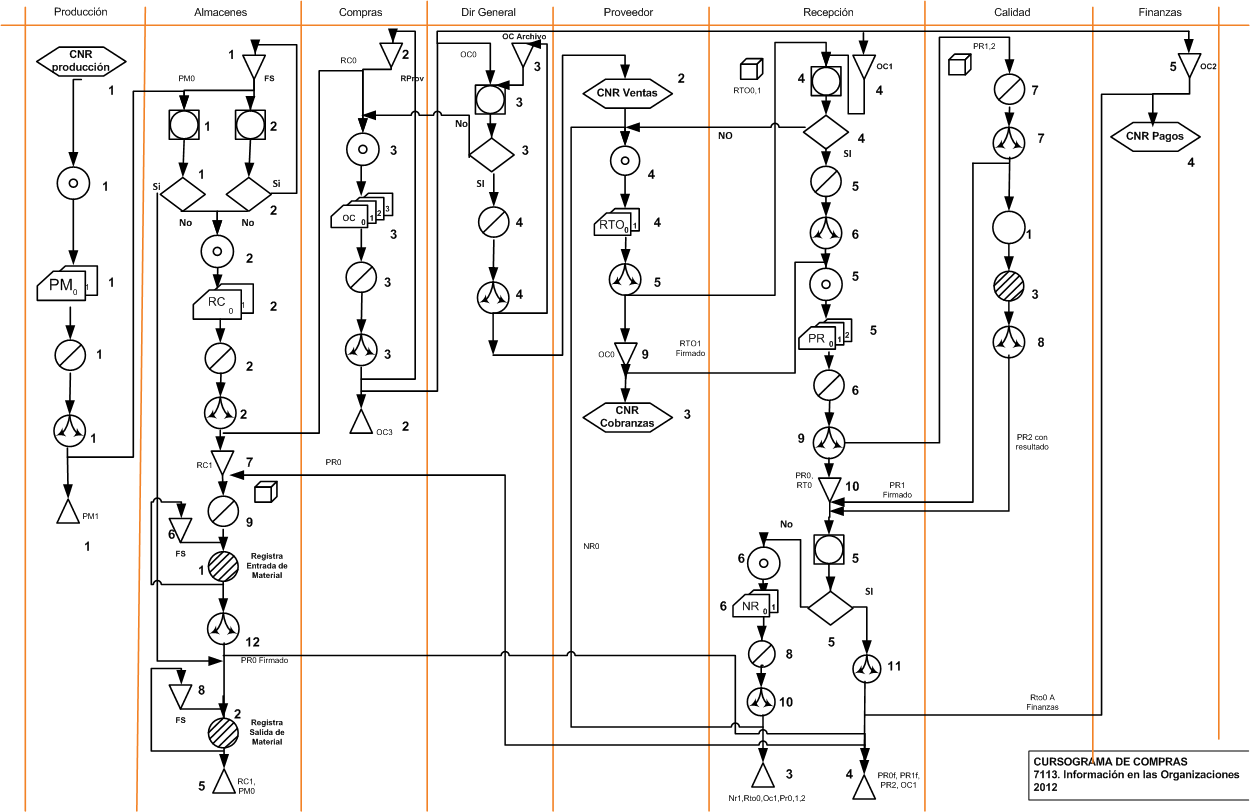
\includegraphics [scale=0.5 ,angle=90]{Empresa/Circuitos/Compras/Compras-manual.png}


\pagebreak
\section{Manual del Cursograma de Compras}
\begin{center}\textbf{Sectores intervinientes}\end{center}
\begin{itemize}
  \item Producci\'on
  \item Almacenes
  \item Compras
  \item Direcci\'on General
  \item Proveedor
  \item Recepci\'on
  \item Control de Calidad
  \item Finanzas
\end{itemize}

\begin{center}
  \textbf{Documentos}
  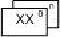
\includegraphics{./Images/Simbolos/simbolo-Documentos.png}
\end{center}
\begin{enumerate}
  \item Pedido de Materiales (PM)
  \item Requerimiento de Compra (RC)
  \item Orden de Compra (OC)
  \item Remito (RTO)
  \item Parte de Recepción (PC)
  \item Nota de Reclamo (NR)
\end{enumerate}

\begin{center}
  \textbf{Emisión de Documentos}
  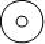
\includegraphics{./Images/Simbolos/simbolo-Emision-de-Documentos.png}
\end{center}
\begin{enumerate}
  \item Producción emite Pedido de Materiales por duplicado
  \item Almacenes emite Requerimiento de Compras por duplicado
  \item Compras emite Orden de Compra por cuadruplicado
  \item El Proveedor emite Remito por duplicado
  \item Recepción emite el Parte de Recepción por triplicado
  \item Recepción emite Nota de Reclamo por duplicado
\end{enumerate}

\begin{center}
  \textbf{Firma}
  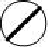
\includegraphics{./Images/Simbolos/simbolo-Firma.png}
\end{center}
\begin{enumerate}
  \item Producción firma Pedido de Materiales.
  \item Almacenes firma Requerimiento de Compra.
  \item Compras firmas las Ordenes de Compra.
  \item Dirección General firma la Orden de Compra.
  \item Recepción firma el Remito del proveedor.
  \item Recepción firma el original del Parte de Recepción.
  \item Calidad firma la copia del Parte de Recepción.
  \item Recepción firma la Nota de Reclamo.
  \item Almacenes firma el Parte de Recepción.
\end{enumerate}

\begin{center}
  \textbf{Distribución}
  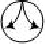
\includegraphics{./Images/Simbolos/simbolo-Distribucion.png}
\end{center}
\begin{enumerate}
  \item Producción distribuye el Pedido de Materiales a Almacenes.
  \item Almacenes distribuye el Requerimiento de Compra a Compras.
  \item Compras distribuye las Ordenes de Compra a Dirección General, Recepción y Finanzas.
  \item Dirección General distribuye la Orden de Compra al Proveedor.
  \item El Proveedor distribuye el Remito a Recepción.
  \item Recepción distribuye el Remito al Proveedor.
  \item Calidad distribuye la copia 1 del Parte de Recepción a Recepción.
  \item Calidad distribuye la copia 2 del Parte de Recepción a Recepción.
  \item Recepción distribuye el Parte de Recepción a Calidad.
  \item Recepción distribuye la Nota de Reclamo al Proveedor.
  \item Recepción distribuye el Remito a Finanzas y el Parte de Recepción a Almacenes.
  \item Almacenes distribuye el Parte de Recepción firmado a Recepción.
\end{enumerate}

\begin{center}
  \textbf{Almacenamiento Transitorio}
  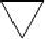
\includegraphics{./Images/Simbolos/simbolo-Almacenamiento-Transitorio.png}
\end{center}
\begin{enumerate}
  \item Almacenes almacena la Ficha de Stock.
  \item Compras almacena el Registro de Proveedores.
  \item Dirección General almacena el Archivo de Ordenes de Compra.
  \item Recepción almacena la copia de la Orden de Compra.
  \item Finanzas almacena el triplicado de la Orden de Compra.
  \item Almacenes almacena la ficha de stock.
  \item Almacenes almacena la copia del Requerimiento de Compra.
  \item Almacenes almacena la ficha de stock.
  \item El Proveedor almacena la Orden de Compra original.
  \item Recepción almacena el Parte de Recepción original y el Remito original.
\end{enumerate}

\begin{center}
  \textbf{Control y verificación}
  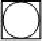
\includegraphics{./Images/Simbolos/simbolo-Control-y-Verificacion.png}
\end{center}
\begin{enumerate}
  \item Almacenes controla si cuenta con stock para satisfacer el Pedido de Materiales.
  \item Almacenes controla si se alcanzó el punto de pedido
  \item Dirección General controla los precios de la Orden de Compra contra Ordenes de Compra archivadas.
  \item Recepción controla la cantidad de materiales recibidos contra lo descripto en la Orden de Compra.
  \item Recepción controla el resultado del control de calidad en el Parte de Recepción.
\end{enumerate}

\begin{center}
  \textbf{Decisión}
  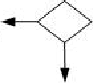
\includegraphics{./Images/Simbolos/simbolo-Decision.png}
\end{center}
\begin{enumerate}
  \item Si Almacenes cuenta con stock para satisfacer el pedido lo despacha; si no, emite Requerimiento de Compra.
  \item Si hay stock por encima del punto de pedido, se actaliza la ficha de stock; si no, Almacenes emite Requerimiento de Compra.
  \item Si Dirección General aprueba la compra firma la Orden de Compra; si no la devuelve a Compras para que la revise.
  \item Si Recepción determina que las cantidades declaradas en el Remito son correctas, lo firma y devuelve al Proveedor; si no, devuelve al Proveedor el Remito y no acepta la mercadería.
  \item Si el control de calidad fue aprobado, Recepción envía el Remito a Finanzas y los materiales a Almacenes; si no, emite Nota de Reclamo y envía al Proveedor.
\end{enumerate}

\begin{center}
  \textbf{Registro}
  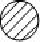
\includegraphics{./Images/Simbolos/simbolo-Registro.png}
\end{center}
\begin{enumerate}
  \item Almacenes registra la entrada de materiales en la ficha de stock.
  \item Almacenes registra la salida de materiales en la ficha de stock.
  \item Calidad registra el resultado del control de calidad en el Parte de Recepción.
\end{enumerate}

\begin{center}
  \textbf{Almacenamiento definitivo}
  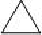
\includegraphics{./Images/Simbolos/simbolo-Almacenamiento-Definitivo.png}
\end{center}
\begin{enumerate}
  \item Producción almacena Pedido de Materiales.
  \item Compras almacena el triplicado de la Orden de Compra.
  \item Recepción almacena el duplicado de la Nota de Reclamo, el original del Remito, el duplicado de la Orden de Compra, y todas las copias del Parte de Recepción
  \item Recepción almacena el original del Parte de Recepción firmado, su duplicado firmado, el triplicado y el original de la Orden de Compra
  \item Almacenes almacena el duplicado del Requerimiento de Compra y el original del Pedido de Materiales
\end{enumerate}

\begin{center}
  \textbf{Circuito no relevado}
  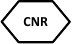
\includegraphics{./Images/Simbolos/simbolo-CNR.png}
  % simbolo-CNR.png: 73x44 pixel, 96dpi, 1.93x1.16 cm, bb=0 0 55 33
\end{center}
\begin{enumerate}
  \item Producción
  \item Ventas (circuito del Proveedor)
  \item Cobranzas (circuito del Proveedor)
  \item Pagos
\end{enumerate}

\pagebreak
\section{Formularios de Compras}
\subsection{Orden de Compra}
\begin{center}
 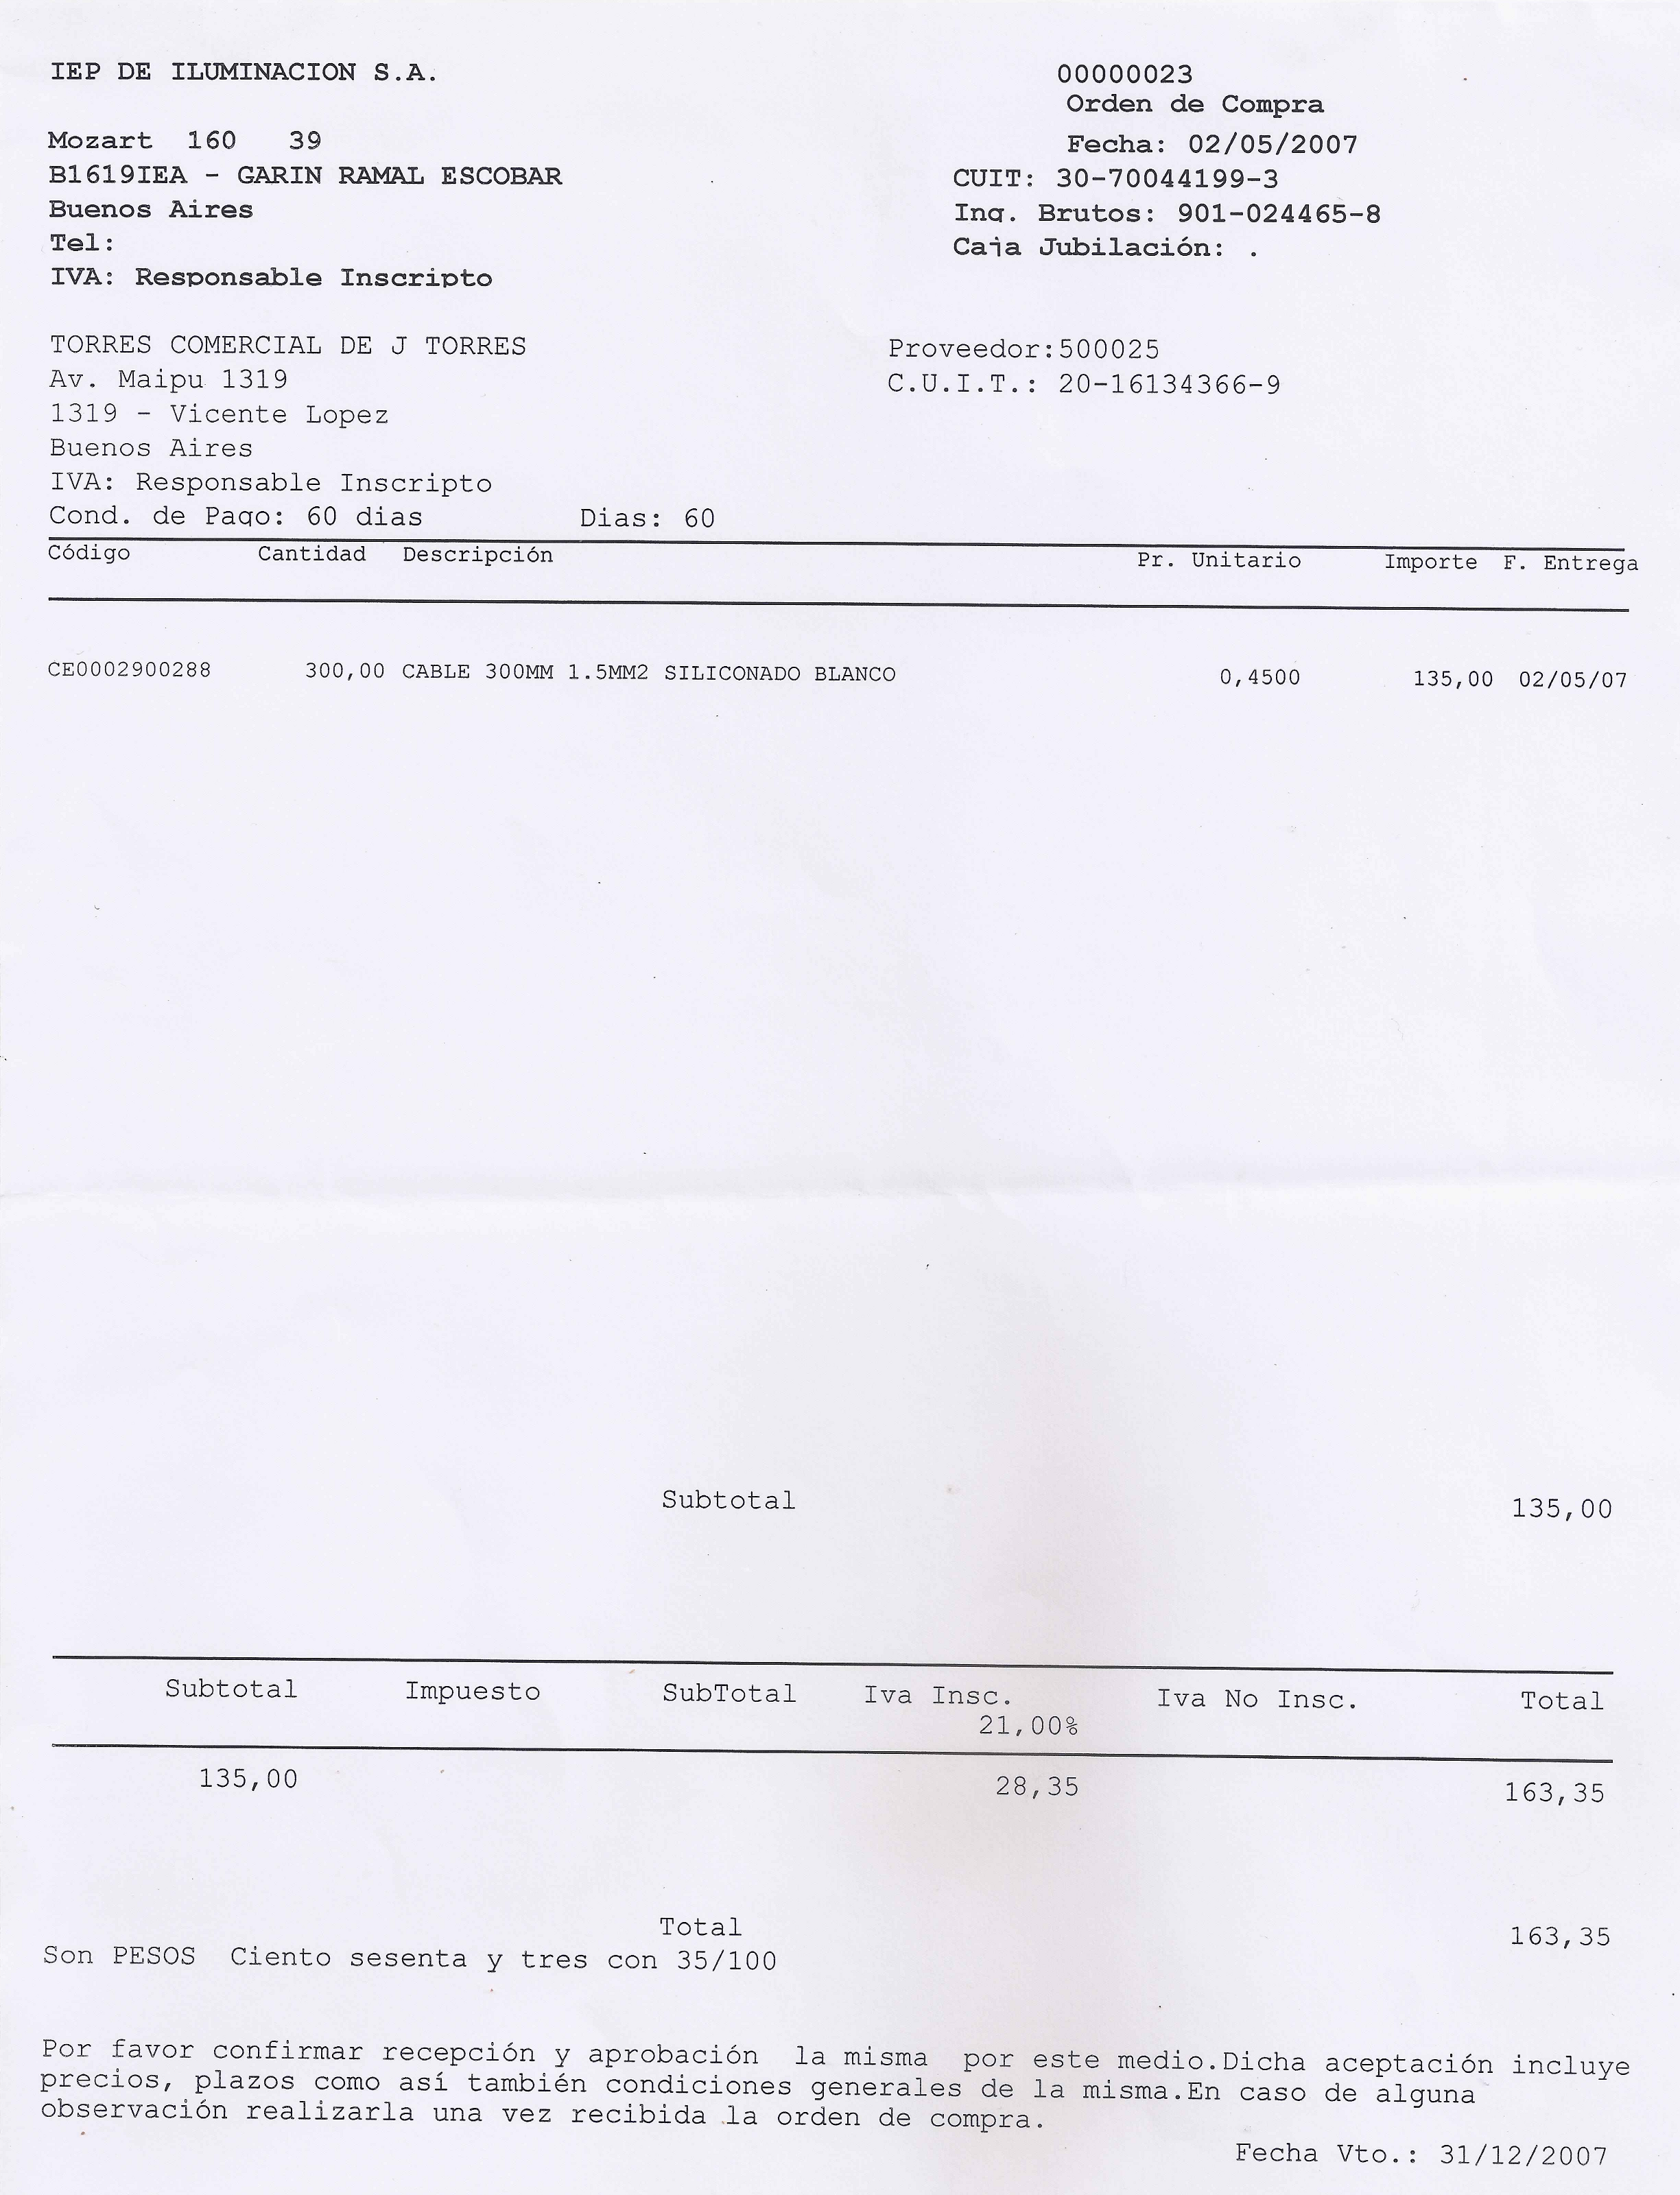
\includegraphics[scale=3.2, keepaspectratio=true]{./Images/FormulariosIEP/Orden-de-Compra.png}
 % Orden-de-Compra.png: 750x1002 pixel, 96dpi
\end{center}
\begin{itemize}
  \item \textbf{Objetivo:} Mediante este documento se comunica al proveedor la decisión de realizar una compra de materiales. Se especifican los productos a comprar con detalle de precios, cantidades, impuestos y condiciones de pago acordes a la previa cotización del proveedor.
  \item \textbf{Alcance:} Es un documento externo, entre la empresa y su proveedor.
  \item \textbf{Emisor:} Compras.
  \item \textbf{Cantidad de Copias Emitidas:} Original y cuatro copias.
  \item \textbf{Sector receptor:} Original a Dirección General para su autorización; primera copia a Recepci\'on; segunda copia a Finanzas; tercera copia a Control de Calidad; y la \'ultima copia a Compras.
 \end{itemize}
\subsubsection{Descripci\'on campos de la Orden de Compra}
\begin{enumerate}
  \item Empresa emisora: Raz\'on Social de la empresa.
  \item Empresa emisora: Informaci\'on de Sucursal. Domicilio y N\'umero de Tel\'efono.
  \item Empresa emisora: Responsabilidad frente al IVA.
  \item Número de Orden de Compra.
  \item Fecha de emisi\'on.
  \item Empresa emisora: CUIT y C\'odigo de Ingresos Brutos.
  \item Proveedor: Raz\'on Social.
  \item Proveedor: Domicilio.
  \item Proveedor: Responsabilidad frente al IVA.
  \item Condici\'on de pago.
  \item C\'odigo del proveedor al que se le compra.
  \item Proveedor: CUIT.
  \item Detalle de la Orden de Compra: C\'odigo del proveedor del \'item.
  \item Detalle de la Orden de Compra: Cantidad solicitada.
  \item Detalle de la Orden de Compra: Descripci\'on del \'item.
  \item Detalle de la Orden de Compra: Precio unitario del \'item.
  \item Detalle de la Orden de Compra: Importe total del \'item (cantidad * precio unitario).
  \item Detalle de la Orden de Compra: Fecha de entrega del \'item.
  \item Detalle de la Orden de Compra: Subtotal de items (suma de los totales de \'item).
  \item Resumen de la Orden de Compra: Subtotal de items (suma de los totales de \'item).
  \item Resumen de la Orden de Compra: Importe de impuestos que aplican (opcional).
  \item Resumen de la Orden de Compra: Subtotal después de impuestos (sólo si aplica impuestos).
  \item Resumen de la Orden de Compra: Gravamen de IVA para Inscriptos.
  \item Resumen de la Orden de Compra: Gravamen de IVA para No Inscriptos.
  \item Resumen de la Orden de Compra: Total después de IVA.
  \item Importe Total de la Orden de Compra.
  \item Importe Total de la Orden de Compra en letras.
  \item Fecha de Vencimiento de la Orden de Compra.
  \item Términos de confirmación de aprobación o rechazo.
\end{enumerate}

\pagebreak
\subsection{Requerimiento de Compra}
\begin{center}
 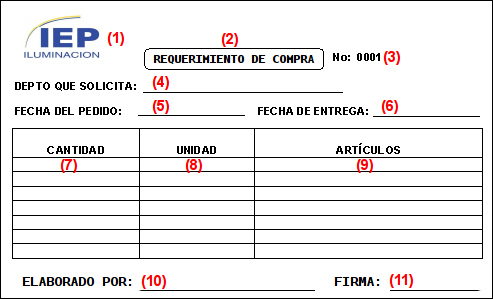
\includegraphics{Images/FormulariosIEP/Requerimiento-de-Compra.png}
 % Requerimiento-de-Compra.png: 493x299 pixel, 96dpi, 13.04x7.91 cm, bb=0 0 370 224
\end{center}

\begin{itemize}
  \item \textbf{Objetivo:} Un Requerimiento de Compra es un pedido interno entre sectores, para que el responsable de compras provea de algún elemento que un sector necesita.
  \item \textbf{Alcance:} Documento interno de la empresa.
  \item \textbf{Emisor:} Almacenes.
  \item \textbf{Cantidad de Copias Emitidas:} Original y copia.
  \item \textbf{Sector receptor:} Original a Compras; y la copia para Almacenes.
 \end{itemize}
\subsubsection{Descripci\'on campos del Requerimiento de Compra}
\begin{enumerate}
 \item Logo de la empresa.
 \item Nombre del formulario.
 \item N\'umero del Requerimiento de Compra.
 \item Departamento que solicita la Compra.
 \item Fecha en la que se realiza el Requerimiento de Compra.
 \item Fecha en la que se necesita los art\'iculos solicitados.
 \item Cantidad solicitada de un art\'iculo.
 \item Unidad de medida de un art\'iculo.
 \item Descripci\'on de un art\'iculo deseado.
 \item N\'umero del proveedor preferido (opcional).
 \item Firma del emisor.
\end{enumerate}


\pagebreak
\section{Normas de Control Interno de Compras}
\begin{itemize}

 \item	{\bf Separaci\'on de funciones: } La función de compras debe estar separada del manejo físico de los bienes y de la registración de los mismos. Compras por lo tanto debe estar separada de los sectores de
Almacenes, Recepción y Finanzas.

 \item	{\bf Iniciación del trámite de compras: } Respaldo de un pedido formal debidamente autorizado.

 \item	{\bf Obtención de un número determinado de cotizaciones: } Los
pedidos y las cotizaciones se realizan por escrito. En compras usuales a proveedores con historial satisfactorio suelen efectuarse las compras en forma directa.

 \item	{\bf Autorización de la compra: } Lo realiza la persona responsable, una vez tomada la decisión de compra; quien la tomó debe intervenir con su firma la orden de compra.

 \item	{\bf Punto de pedido: } La cantidad en existencia a partir de la cual se debe solicitar la compra de un articulo, se establece como un stock mínimo, teniendo en cuenta el programa de producción vigente.

 \item	{\bf Control de la mercadería recibida: } De la cantidad y la calidad. La función de Calidad requiere de conocimientos técnicos, por lo cual está separada de Recepción, que en el
momento de la recepción solo da conformidad por la cantidad.

 \item	{\bf Constitución de seguros sobre mercaderías en tránsito }
 
 \item	{\bf Prenumeración de formularios: } En forma preimpresa y correlativa para Requerimiento de Compra y Orden de
Compra. Controles de correlatividad de
los formularios utilizados.

\end{itemize}
